\chapter{Белый шум}
\label{ch:chap2}

\textbf{Что такое белый (гауссовский) шум?}

Белый шум (гауссовский шум) - простейший случайный процесс, который представляет собой последовательность
некоррелированных случайных переменных с нормальным распределением. Эргодичен и стационарен.

\textbf{Что такое эргодичный случайный процесс?}

Эргодичный случайный процесс - случайный процесс, у которого среднее по времени и ансамблю в теории совпадают (при бесконечном числе измерений),
но на деле немного отличаются, т.к бесконечное число измерений получить невозможно.

\textbf{Что такое среднее по ансамблю?}

Среднее по ансамблю - это математическое ожидание случайного процесса, вычисленное по множеству разных реализаций (ансамблю) 
в фиксированный момент времени. Иными словами: у нас есть мн-во реализаций процесса (выборок) для одного и того же отсчета
(момента времени), допустим для отсчета n = 3. Мы суммируем все значения реализаций в момент времени n = 3 и делим на 
общее кол-во реализаций. Это и будет средним по ансамблю. При вычислении нужно суммировать строки.

\textbf{Что такое среднее по времени?}

Среднее по ансамблю - это математическое ожидание случайного процесса, вычисленное по множеству разных отсчетов (моментов времени) 
в фиксированной реализации (выборке). Иными словами: у нас есть единственная реализация в разные моменты времени. Мы суммируем
значения СП во все моменты времени и делим на кол-во отсчетов (моментов времени). При вычислении суммируем столбцы.

\textbf{Что нам дает эргодичность?}

Часто необходимо знать, как будет себя вести случайный процесс, но это достаточно сложно, т.к процесс все-таки случаен и будет
вести себя в каждой выборке по-разному. Если СП обладает таким свойством, как эргодичность, то это во многом упрощает эту задачу,
т.к среднее по реализациям (ансамблю) равно среднему по времени (в теории), т.е мы можем взять всего одну реализацию (выборку) и 
ее среднее (мат.ожидание) будет одинаковым (в теории) для всех реализаций. 

\textbf{Что такое стационарность СП?}

Стационарность — это свойство случайного процесса, при котором его статистические характеристики не зависят от времени.
Процесс называется стационарным в строгом смысле, если его любые вероятностные характеристики не зависят от сдвига во времени.
Процесс называется стационарным в слабом смысле, если математическое ожидание, дисперсия и коварицация (при условии, что она зависит
только от лага (разности во времени)) не зависят от сдвига во времени. Любой эргодический процесс - стационарен, но не каждый
стационарный процесс эргодичен.

Реализация:\\

\begin{figure}[H]
    \centering
    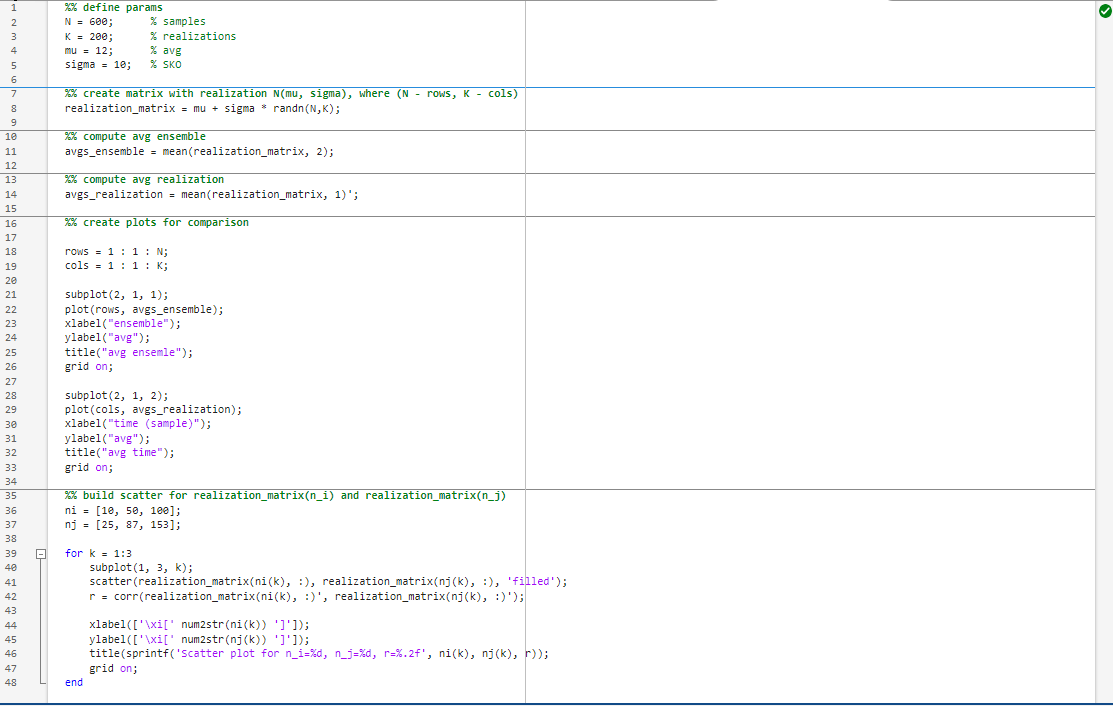
\includegraphics[width=1.0\textwidth]{white_noise_real.png}
    \caption{Реализация задания для белого шума}
\end{figure}

Результат:\\

\begin{figure}[H]
    \centering
    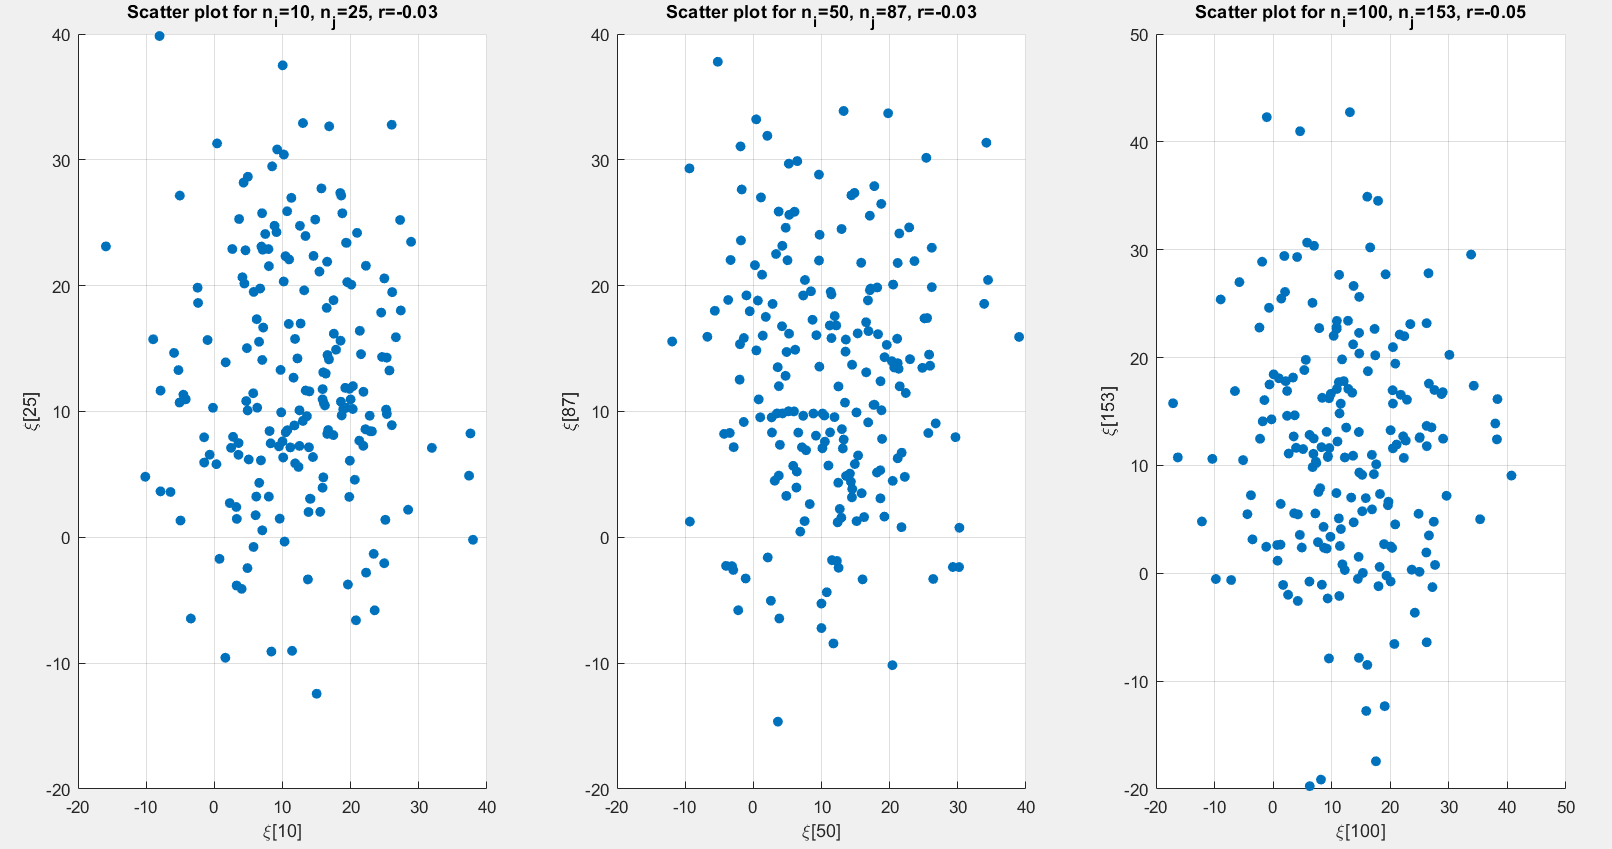
\includegraphics[width=1.0\textwidth]{white_noise_result.png}
    \caption{Результат задания для белого шума}
\end{figure}

Сверху изображена диаграмма рассеяния, где показана зависимость между реализациями процесса в разные моменты времени. Точки расположены
хаотично, что указывает на то, что в каждый момент времени все реализации некоррелированные, т.е поведение одной реализации
не зависит от поведения другой (что и сказано в определении белого шума). Над каждым графиком указана коореляция, которая почти равна нулю,
что подтверждает выше сказанное.

\endinput